% Provenance (never printed): see sources/outline_sources.md (Year 3: the
% structure of the Galaxy; the rotation curve and dark matter; galaxy types;
% the distance ladder, Hubble's law recalled from the physics books).
% Brief: sources/book5/BRIEFS.md, ch. 29. Curves from figdata/bachelor-3/
% rotation_curve.py (the circular velocity curve of Eilers et al. 2019 with the
% Pouliasis et al. 2017 Model I baryons and an NFW halo fitted to it) and
% distance_ladder.py (the OGLE-IV Cepheids of the Large Magellanic Cloud, CDS
% J/AcA/65/297, and the ranges of the rungs). Exercise and problem values in the
% Book 5 scratch calculator calc/ch29.py. The survey of Part I of the problem and
% the galaxies of the exercises are invented.
\chapter{De Melkweg en sterrenstelsels}\label{ch:b3:milky-way-galaxies}

In het zonnestelsel bewegen de planeten die ver van de Zon staan langzaam: Mercurius
draait eromheen met \qty{47.4}{km.s^{-1}}, Neptunus met \qty{5.4}{km.s^{-1}}, zoals
de derde wet van Kepler voor lichamen die door één centrale massa worden vastgehouden vereist. De sterren
van de Melkweg gedragen zich niet zo. Gemeten aan de bewegingen van meer
dan twintigduizend rode reuzen bedraagt de snelheid van hun cirkelvormige banen
\qty{227}{km.s^{-1}} op \qty{5}{kpc} van het centrum, \qty{229}{km.s^{-1}}
bij de Zon, en nog steeds \qty{198}{km.s^{-1}} op \qty{25}{kpc}, waar nauwelijks
sterren of gas meer aanwezig zijn. Als de massa die we zien het enige was wat er is, zouden de buitenste
sterren veel trager zijn. Iets onzichtbaars houdt ze vast. Dit hoofdstuk
beschrijft de Melkweg waarin we leven, bepaalt de massa uit haar rotatie, ordent de
andere sterrenstelsels in typen en beklimt de keten van methoden waarmee
hun afstanden en de uitdijing van het heelal worden gemeten.
% ledger: planet:Mercury.vorb, planet:Neptune.vorb, eilers19:vc, eilers19:table1

\begin{recall}
De Melkweg, het Doppler-effect, de wetten van Kepler, de stelling van Newton over de
aantrekking van een bolvormige schil, donkere materie, zwarte gaten en hun
Schwarzschildstraal, supernova's, witte dwergen, de 21-cm-lijn van atomair
waterstof en de wet van Hubble staan in de natuurkundeboeken. De jaarlijkse parallax,
de parsec, flux en lichtkracht, schijnbare en absolute magnitude, de
afstandsmodulus, fotometrische banden en de kleurindex staan in
Boek~3, in het hoofdstuk over telescopen en fotometrie. Het
interstellaire medium en het stof erin staan in Boek~4, in het hoofdstuk
over het interstellaire medium en stervorming.
\end{recall}

\section{De structuur van de Melkweg}\label{sec:b3:milky-way-galaxies:structure}

Vanaf de Aarde gezien is het Melkwegstelsel de Melkweg: een lichtband rond
de hele hemel, doorkruist door donkere stofbanen en het helderst in de richting van
het sterrenbeeld Boogschutter, waar het centrum ligt. De band is de schijf waarin de Zon zit,
van binnenuit langs de rand gezien.

\begin{omfigure}
\centering
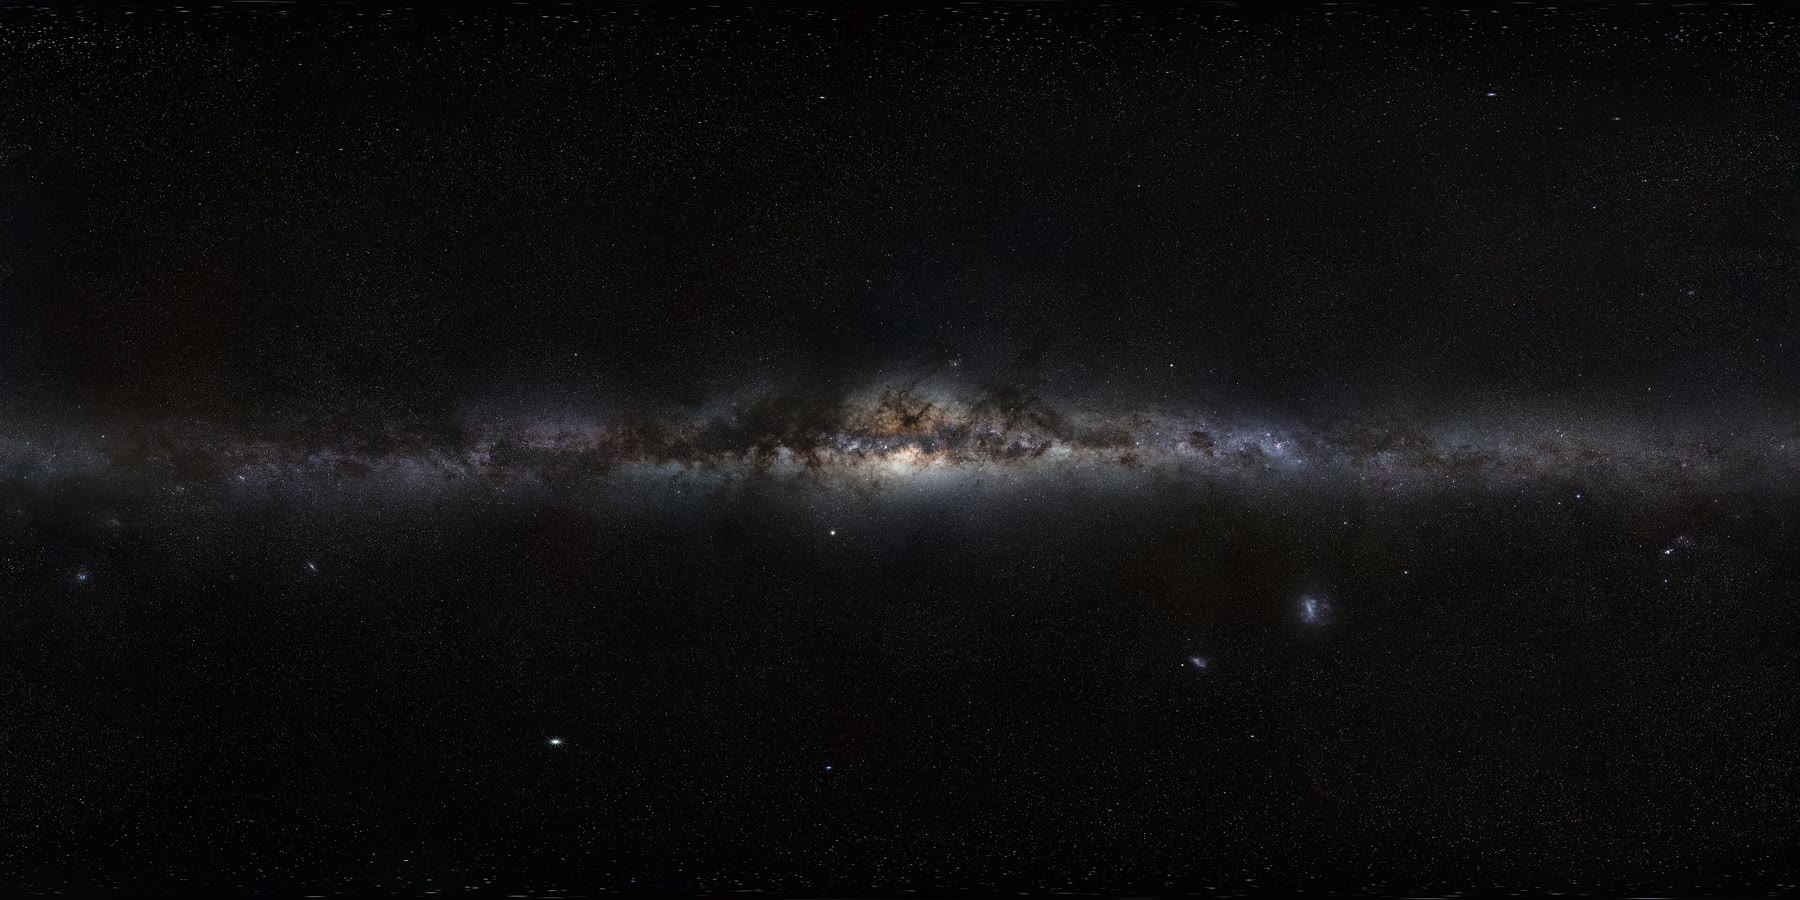
\includegraphics[width=0.96\linewidth]{images/book5/b3-milky-way-panorama.jpg}
\par\smallskip{\small De hele hemel in één beeld, geprojecteerd zo dat het
vlak van de Melkweg dwars door het midden loopt en het centrum in het
midden van het beeld ligt. De band is de schijf van binnenuit gezien; de donkere
stroken zijn stof in de schijf dat de sterren erachter verbergt; de centrale bulge
zwelt rond het centrum op. De twee kleine vlekjes onder de band, rechts
zijn de Grote en de Kleine Magellaanse Wolk, twee satellietsterrenstelsels;
de zwakke vlek onder de band bij de linkerrand is het
Andromedastelsel. Foto ESO/S.~Brunier, CC BY~4.0.}\label{fig:b3:milky-way-galaxies:panorama}
\end{omfigure}
% ledger: photo:b3-milky-way-panorama, mcconn12:local-group

\begin{definition}[Galactische schijf, dikke schijf, bulge en stellaire halo]\label{def:b3:milky-way-galaxies:structure}
De \emph{galactische schijf}\index{galactische schijf} is het afgeplatte deel van
de Melkweg, opgebouwd uit sterren, gas en stof in bijna cirkelvormige banen rond
het centrum; de dichtheid neemt ongeveer exponentieel af met de hoogte boven het
middenvlak en met de afstand tot het centrum, over een schaalhoogte en een
schaallengte. De \emph{dikke schijf}\index{dikke schijf} is een tweede, oudere
schijfcomponent met een grotere schaalhoogte en een kleinere massa. De
\emph{galactische bulge}\index{galactische bulge} is de centrale concentratie van
sterren die uit de schijf opzwelt. De \emph{stellaire halo}\index{stellaire halo}
is het ijle, ruwweg sferoïdale onderdeel van oude sterren en
bolvormige sterrenhopen die de schijf en de bulge omringt.
\end{definition}

De Melkweg is een balkspiraal. In de omgeving van de Zon heeft de dunne
schijf een schaalhoogte van ongeveer \qty{300}{pc} en de \omterm{def:b3:milky-way-galaxies:structure}{dikke schijf} van
ongeveer \qty{900}{pc}; hun schaallengten zijn ongeveer \qty{2.6}{kpc} en
\qty{2.0}{kpc}. De \omterm{def:b3:milky-way-galaxies:structure}{dikke schijf} bevat ongeveer \num{6e9} zonsmassa's,
ruwweg een vijfde van de dunne schijf. Van opzij gezien is de bulge een doos
of een pinda: het is het verdikte binnenste deel van een balk van sterren van ongeveer
\qty{5}{kpc} in halve lengte, waarvan de lange as een hoek maakt van
\ang{27} met de lijn van de Zon naar het centrum. De \omterm{def:b3:milky-way-galaxies:structure}{stellaire halo} bevat
slechts ongeveer één procent van de sterren. Samen wegen de sterren van de Melkweg
ongeveer \num{5e10} zonsmassa's.
% ledger: bhg16:structure

\begin{omfigure}
\centering
\begin{tikzpicture}[x=0.17cm, y=0.17cm, font=\scriptsize]
% edge-on view
\begin{scope}
\fill[omProp!8] (0,0) circle (17);
\draw[omProp!60, densely dotted] (0,0) circle (17);
\fill[black!12] (0,0) ellipse (15 and 2.4);
\fill[black!30] (0,0) ellipse (15 and 0.8);
\fill[black!45] (-3.2,0) .. controls (-3.4,2.3) and (-1.2,2.0) .. (0,1.4)
  .. controls (1.2,2.0) and (3.4,2.3) .. (3.2,0)
  .. controls (3.4,-2.3) and (1.2,-2.0) .. (0,-1.4)
  .. controls (-1.2,-2.0) and (-3.4,-2.3) .. (-3.2,0) -- cycle;
\foreach \p in {(-10,9),(6,12),(12,-7),(-6,-13),(-13,-4),(3,-9),(12,8)}
  \fill[omProp] \p circle (0.35);
\fill[ocYellow, draw=black] (-8.2,0.15) circle (0.55);
\node[anchor=south] at (-8.2,0.9) {Zon};
\draw[|<->|] (0,-4.6) -- node[below] {$R_0 \approx \qty{8.2}{kpc}$} (-8.2,-4.6);
\node[anchor=west] at (15.3,0) {dunne schijf};
\node[anchor=west] at (13.2,2.8) {dikke schijf};
\draw[->] (4.6,4.6) node[anchor=south west, inner sep=1pt] {bulge} -- (2.4,1.7);
\node[omProp!80!black] at (-11,13.5) {stellaire halo};
\node at (0,-19.5) {(a) langs de rand gezien};
\end{scope}
% face-on view
\begin{scope}[xshift=7.6cm]
\fill[omProp!8] (0,0) circle (17);
\draw[omProp!60, densely dotted] (0,0) circle (17);
\fill[black!12] (0,0) circle (15);
\foreach \a in {0,180} {
  \draw[line width=1.6pt, black!40, rotate=\a+63]
    plot[domain=0:3.9, samples=50] ({5*exp(0.25*\x)*cos(\x r)}, {5*exp(0.25*\x)*sin(\x r)});
}
\fill[black!45, rotate=63] (0,0) ellipse (5 and 1.5);
\draw[dashed] (0,0) circle (8.2);
\fill[ocYellow, draw=black] (0,-8.2) circle (0.55);
\node[anchor=north] at (0,-8.9) {Zon};
\draw[dotted, thick] (0,0) -- (0,-8.2);
\draw[thick, ->] (0,0) ++(25:16) arc (25:-25:16);
\node[anchor=west] at (17.3,0) {rotatie};
\node[anchor=west, fill=black!12, inner sep=1pt] at (3.4,3.4) {balk};
\draw[|-|] (6,-15.5) -- node[below] {\qty{5}{kpc}} (11,-15.5);
\node at (0,-19.5) {(b) vanaf de noordelijke galactische pool gezien};
\end{scope}
\end{tikzpicture}
\par\smallskip{\small Schets van de Melkweg, op schaal voor de belangrijkste
afmetingen. (a)~Langs de rand gezien: de dunne schijf (donkere band), de \omterm{def:b3:milky-way-galaxies:structure}{dikke schijf} (lichte
band), de doosvormige bulge, en de \omterm{def:b3:milky-way-galaxies:structure}{stellaire halo} met haar bolvormige
sterrenhopen (oranje stippen); de Zon staat in de schijf, ongeveer \qty{8.2}{kpc}
van het centrum en ongeveer \qty{25}{pc} boven het middenvlak (te klein om
weer te geven). (b)~Vanaf de noordelijke galactische pool gezien: de balk, ongeveer
\qty{5}{kpc} in halve lengte, gekanteld over \ang{27} ten opzichte van de lijn van de Zon
naar het centrum (gestippeld); de zonnecirkel (gestreept); spiraalarmen schematisch
getekend; de Melkweg draait in deze weergave met de klok mee.}\label{fig:b3:milky-way-galaxies:sketch}
\end{omfigure}
% ledger: bhg16:structure, gravity19:r0

\begin{definition}[Sterpopulatie]\label{def:b3:milky-way-galaxies:populations}
Een \emph{sterpopulatie}\index{sterpopulatie} is een groep sterren
van een sterrenstelsel die een bereik van ouderdommen, chemische samenstellingen en
banen delen. De jonge sterren van de dunne schijf, rijk aan elementen zwaarder dan
helium en op bijna cirkelvormige banen, worden traditioneel
populatie~I genoemd; de oude sterren van de halo en van de bolvormige sterrenhopen, arm
aan zware elementen en op banen met grote willekeurige bewegingen en weinig netto rotatie,
populatie~II.
\end{definition}

De \omterm{def:b3:milky-way-galaxies:structure}{dikke schijf} ligt daartussen: haar sterren zijn meestal ouder dan die van
de dunne schijf en zijn bij een gegeven ijzergehalte rijker aan de lichte elementen
die sterrenkundigen alfa-elementen noemen, gemeten ten opzichte van ijzer. De
\omterm{def:b3:milky-way-galaxies:structure}{stellaire halo} is een
fossiel archief: een groot deel ervan is opgebouwd uit kleine sterrenstelsels die in
de Melkweg vielen en door haar getijden uiteengereten werden, en sommige van hun
sterrenstromen zijn nog steeds over de hemel te volgen.
% ledger: bhg16:populations

\begin{definition}[Galactische coördinaten]\label{def:b3:milky-way-galaxies:coordinates}
De \emph{galactische coördinaten}\index{galactische coördinaten} van een richting
zijn de \emph{galactische breedte} $b$, de hoek ten opzichte van het galactische vlak
(positief richting de noordelijke galactische pool), en de \emph{galactische
lengte} $\ell$, gemeten in het vlak vanaf de richting van het
Galactisch Centrum ($\ell = 0$) via $\ell = \ang{90}$, de richting
waarheen de rotatie van de Melkweg de Zon meevoert. Het vlak werd
in 1958 vastgelegd als het hoofdvlak van het atomaire waterstof van de Melkweg;
de noordelijke galactische pool ligt op rechte klimming \ang{192.25}
($12^\mathrm{h}49^\mathrm{m}$) en declinatie \ang{27.4} (equinox
1950).
\end{definition}
% ledger: liu11:galactic, reid20:sgra

De Zon ligt niet helemaal in het vlak: zij ligt zo'n \qty{25}{pc} ten noorden ervan.
Haar afstand tot het centrum, $R_0$, was lange tijd het meest onzekere getal van
de galactische sterrenkunde. Ze wordt nu geometrisch gemeten: de ster S2 draait om
het centrale zwarte gat van de Melkweg met een omlooptijd van \num{16} jaar, waarvan de
hoekgrootte op de hemel en de snelheid langs de zichtlijn, gevolgd
gedurende 27 jaar, de afstand tot het centrum rechtstreeks geven:
$R_0 = \qty{8178}{pc}$, met een statistische fout van \qty{13}{pc} en een systematische
fout van \qty{22}{pc}. Een overzicht van alle methoden geeft
$R_0 = \qty[separate-uncertainty=true]{8.2 \pm 0.1}{kpc}$.
% ledger: bhg16:structure, gravity19:r0

\section{Rotatie en de halo van donkere materie}\label{sec:b3:milky-way-galaxies:rotation}

\begin{definition}[Lokale standaard van rust]\label{def:b3:milky-way-galaxies:lsr}
De \emph{lokale standaard van rust}\index{lokale standaard van rust} (LSR) is
het referentiestelsel dat zich beweegt op de cirkelvormige baan om het Galactisch
Centrum die door de huidige positie van de Zon loopt. Snelheden van nabije
sterren en gas worden ten opzichte ervan opgegeven.
\end{definition}

De Zon beweegt ten opzichte van de LSR met ongeveer \qty{10}{km.s^{-1}} richting het
Galactisch Centrum, \qty{11}{km.s^{-1}} in de richting van de rotatie en
\qty{7}{km.s^{-1}} richting de noordelijke galactische pool: een kleine peculiaire
beweging bovenop een baan met een snelheid $V_0$ van enkele honderden kilometers
per seconde. Vanaf de Aarde gezien verschuift de radiobron in het centrum van de
Melkweg langs het galactische vlak met \qty{6.411}{mas} per jaar; bijna
de hele verschuiving is de weerspiegeling van de baan van de Zon, en die geeft de
totale snelheid om het centrum, \qty[separate-uncertainty=true]{248 \pm 3}{km.s^{-1}}
(zie \cref{exo:b3:milky-way-galaxies:2}).
% ledger: bhg16:lsr, reid20:sgra

\begin{definition}[Rotatiekromme; Oort-constanten]\label{def:b3:milky-way-galaxies:rotation-curve}
De \emph{rotatiekromme}\index{rotatiekromme} van een schijfstelsel is de
snelheid $V(R)$ van een cirkelvormige baan in zijn vlak als functie van de
afstand $R$ tot zijn centrum. Voor de Melkweg, met $V_0 = V(R_0)$ en
$V'_0 = \mathrm{d}V/\mathrm{d}R$ bij $R_0$, de \emph{Oort-
constanten}\index{Oort-constanten} zijn
\[
A = \frac12\left(\frac{V_0}{R_0} - V'_0\right), \qquad
B = -\frac12\left(\frac{V_0}{R_0} + V'_0\right).
\]
\end{definition}

$A$ meet de afschuiving van de rotatie van de schijf en $B$ de vorticiteit: in een
schijf die als een star lichaam draait geldt $V'_0 = V_0/R_0$ en $A = 0$; bij een vlakke
\omterm{def:b3:milky-way-galaxies:rotation-curve}{rotatiekromme} $A = -B$. Hun verschil is de hoeksnelheid van de LSR,
$A - B = V_0/R_0 = \omega_0$, en hun som is de helling, $A + B = -V'_0$.

\begin{theorem}[Formules van Oort]\label{thm:b3:milky-way-galaxies:oort}
Een ster op een afstand $d \ll R_0$ van de Zon, in het galactische vlak bij
de galactische lengte $\ell$, op een cirkelvormige baan, heeft ten opzichte van de LSR de radiale
snelheid $v_r$ en de transversale snelheid $v_t$ (positief in de
richting van toenemende $\ell$)
\[
v_r = A\,d\sin 2\ell, \qquad v_t = d\,(A\cos 2\ell + B),
\]
in eerste orde in $d/R_0$.
\end{theorem}

\begin{proof}
Laat $\omega(R) = V(R)/R$ de hoeksnelheid van de baan op $R$ zijn. Stel
het Galactisch Centrum in de oorsprong, de Zon op afstand $R_0$, en laat de
ster op afstand $R$ van het centrum liggen, met zijn positie gezien vanuit het
centrum een hoek $\theta$ maken met die van de Zon.
De snelheid van de ster $\omega R$ en de snelheid van de LSR $\omega_0 R_0$ worden op de
zichtlijn geprojecteerd; met wat goniometrie in de driehoek Zon--ster--centrum (de sinusregel
geeft $R\sin(\ell + \theta) = R_0\sin\ell$) levert het exacte resultaat
$v_r = R_0\,[\omega(R) - \omega_0]\sin\ell$. Evenzo, in de richting
loodrecht op de zichtlijn,
$v_t = R_0\,[\omega(R) - \omega_0]\cos\ell - \omega(R)\,d$. Voor een nabije
ster, $\omega(R) - \omega_0 \approx \omega'_0\,(R - R_0)$ en
$R - R_0 \approx -d\cos\ell$. Dan
$v_r \approx -R_0\omega'_0\,d\cos\ell\sin\ell = -\tfrac12 R_0\omega'_0\,
d\sin 2\ell$ en, met behoud van de termen van eerste orde,
$v_t \approx -R_0\omega'_0\,d\cos^2\ell - \omega_0 d$. Met
$\omega'_0 = V'_0/R_0 - V_0/R_0^2$, $-\tfrac12 R_0\omega'_0 = A$ en
$-R_0\omega'_0\cos^2\ell - \omega_0 = A(1 + \cos 2\ell) - (A - B) =
A\cos 2\ell + B$.
\end{proof}

De radiële snelheden van nabije sterren variëren dus als $\sin 2\ell$ over
de hemel, en hun eigenbewegingen als $\cos 2\ell$ rond een gemiddelde dat door $B$ wordt bepaald.
Uit de eigenbewegingen en parallaxen van \num{304267} sterren van de eerste
Gaia-catalogus, op een typische afstand van \qty{230}{pc}, de \omterm{def:b3:milky-way-galaxies:rotation-curve}{Oort-constanten}
bedragen $A = \qty[separate-uncertainty=true]{15.3 \pm 0.4}{km.s^{-1}.kpc^{-1}}$
en $B = \qty[separate-uncertainty=true]{-11.9 \pm 0.4}{km.s^{-1}.kpc^{-1}}$.
Twee extra termen die een axisymmetrische schijf niet zou hebben, $C$
en $K$ genoemd, kwamen op ongeveer \qty{-3}{km.s^{-1}.kpc^{-1}} uit: de lokale schijf is
door de balk en de spiraalarmen geroerd.
% ledger: bovy17:oort

\subsection*{De rotatiekromme uit de 21-cm-lijn}

Atomair waterstof vult de schijf en zendt de 21-cm-lijn uit bij
\qty{1420.405751}{MHz}; radiogolven doorkruisen het stof dat de
verre schijf bij zichtbare golflengten verbergt. Langs een zichtlijn
in het vlak voegt elke gaswolk zijn lijn toe bij de Dopplerverschuiving van
zijn radiële snelheid, en het profiel van de lijn is een spectrum van
snelheden. Binnen de zonnecirkel springt één snelheid eruit.
% ledger: nrao:hi-line

\begin{theorem}[Raakpuntmethode]\label{thm:b3:milky-way-galaxies:tangent}
Laat gas bewegen op cirkelbanen met een hoeksnelheid $\omega(R)$ die
naar buiten afneemt. Langs een zichtlijn op lengtegraad
$0 < \ell < \ang{90}$ is de radiële snelheid ten opzichte van de LSR het grootst
in het raakpunt, waar de zichtlijn een baan raakt, op
$R = R_0\sin\ell$, en de grootste waarde ervan is
\[
v_\mathrm{max} = V(R_0\sin\ell) - V_0\sin\ell .
\]
\end{theorem}

\begin{proof}
Volgens het bewijs van de formules van Oort heeft gas op afstand $R$ van het centrum
op de zichtlijn een radiële snelheid $v_r = R_0\,[\omega(R) - \omega_0]\sin\ell$. Met
$\sin\ell > 0$ en $\omega$ afnemend is $v_r$ het grootst waar $R$
het kleinst is. Langs de zichtlijn is $R$ het kleinst aan de voet van de
loodlijn vanuit het centrum, waar $R = R_0\sin\ell$. Daar geldt
$R_0\,\omega(R)\sin\ell = \omega(R)\,R = V(R)$ en
$R_0\,\omega_0\sin\ell = V_0\sin\ell$.
\end{proof}

\begin{omfigure}
\centering
\begin{tikzpicture}[scale=0.95, font=\small]
\coordinate (C) at (0,0);
\coordinate (S) at (0,-4);
\coordinate (T) at (-1.970,-1.653);
\draw[dashed, black!50] (C) circle (4);
\draw[dashed, omDef!70] (C) circle (2.571);
\fill (C) circle (2pt) node[anchor=south west] {Galactisch centrum};
\fill[ocYellow, draw=black] (S) circle (3pt);
\node[anchor=north] at (0,-4.15) {Zon};
\draw[thick] (S) -- ($(S)!2.25!(T)$) node[anchor=south east, fill=white, inner sep=1pt] {zichtlijn};
\draw[dotted, thick] (C) -- (S);
\draw[thick, omThm] (C) -- node[anchor=north west, fill=white, inner sep=1pt, pos=0.45] {$R_0\sin\ell$} (T);
\fill[omThm] (T) circle (2pt);
\node[anchor=north east, omThm, fill=white, inner sep=1pt] at ($(T)+(-0.05,-0.08)$) {raakpunt};
\draw[->, very thick, omDef] (T) -- ++(-0.643*1.3, 0.766*1.3) node[anchor=south west, fill=white, inner sep=1pt] {$V(R)$};
\draw[->, very thick, black!70] (S) -- ++(-1.4,0) node[anchor=north] {$V_0$};
\draw (0,-3.2) arc (90:130:0.8);
\node at (-0.30,-2.85) {$\ell$};
\node[anchor=west] at (0.1,-2.2) {$R_0$};
\node[black!60, anchor=west] at (2.9,-2.9) {zonnecirkel};
\end{tikzpicture}
\par\smallskip{\small De raakpuntmethode, gezien vanaf de noordelijke
galactische pool. Langs een zichtlijn op lengtegraad $\ell$ ligt het gas het dichtst
bij het centrum, in het raakpunt op $R = R_0\sin\ell$ (rood). Zijn
baansnelheid $V(R)$ ligt langs de zichtlijn, en de
radiële snelheid daar is de grootste die het lijnprofiel toont. Elke
lengtegraad levert één punt van de \omterm{def:b3:milky-way-galaxies:rotation-curve}{rotatiekromme} binnen de zonnecirkel op.}\label{fig:b3:milky-way-galaxies:tangent}
\end{omfigure}

De hoogste snelheid in elk 21-cm-profiel levert dus $V$ op bij
$R_0\sin\ell$, en een doorloop van lengtegraden van \ang{0} tot \ang{90} geeft
de \omterm{def:b3:milky-way-galaxies:rotation-curve}{rotatiekromme} van het centrum tot aan de Zon. Voorbij de zonnecirkel
raakt geen zichtlijn aan een baan en faalt de methode:
daar moet de afstand van elke tracer net zo goed gemeten worden als zijn
snelheid. Sinds 2014 heeft een satelliet de parallaxen van meer dan
een miljard sterren gemeten, en de buitenste \omterm{def:b3:milky-way-galaxies:rotation-curve}{rotatiekromme} wordt nu door sterren getraceerd.
% ledger: nrao:hi-line, gaia:dr3

\begin{omfigure}
\centering
\begin{tikzpicture}
\begin{axis}[width=0.90\linewidth, height=0.52\linewidth,
  xmin=0, xmax=26, ymin=0, ymax=265,
  xlabel={afstand tot het galactische centrum $R$ (kpc)}, ylabel={cirkelsnelheid (\unit{km.s^{-1}})},
  tick label style={font=\scriptsize}, label style={font=\small},
  legend style={font=\scriptsize, at={(0.5,-0.16)}, anchor=north, legend columns=4, draw=none, cells={anchor=west}, /tikz/every even column/.append style={column sep=1em}}]
\addplot[thin, black!40, dashed, forget plot] coordinates {(8.122,0) (8.122,265)};
\node[font=\scriptsize, anchor=south west, rotate=90] at (axis cs:7.9,4) {Zon};
\addplot[only marks, mark=*, mark size=1.1pt, black, error bars/.cd, y dir=both, y explicit]
  table[x=R, y=vc, y error minus=sig_lo, y error plus=sig_hi] {figdata/out/bachelor-3-rotation_curve-data.dat};
\addlegendentry{gemeten}
\addplot[very thick, omDef] table[x=R, y=v_tot] {figdata/out/bachelor-3-rotation_curve-model.dat};
\addlegendentry{model totaal}
\addplot[thick, black!55] table[x=R, y=v_bar] {figdata/out/bachelor-3-rotation_curve-model.dat};
\addlegendentry{alle baryonen}
\addplot[thick, dashed, red!70!black] table[x=R, y=v_halo] {figdata/out/bachelor-3-rotation_curve-model.dat};
\addlegendentry{halo van donkere materie}
\addplot[densely dotted, thick, omProp] table[x=R, y=v_bulge] {figdata/out/bachelor-3-rotation_curve-model.dat};
\addlegendentry{bulge}
\addplot[dashdotted, thick, omMeth] table[x=R, y=v_thin] {figdata/out/bachelor-3-rotation_curve-model.dat};
\addlegendentry{dunne schijf}
\addplot[densely dashed, thick, violet!70!black] table[x=R, y=v_thick] {figdata/out/bachelor-3-rotation_curve-model.dat};
\addlegendentry{dikke schijf}
\end{axis}
\end{tikzpicture}
\par\smallskip{\small De \omterm{def:b3:milky-way-galaxies:rotation-curve}{rotatiekromme} van de Melkweg. Stippen: de cirkelsnelheid
gemeten aan rode reuzen tussen 5 en \qty{25}{kpc} (Eilers
en anderen, 2019), met hun foutbalken. Lijnen: de snelheden die de
bulge, de dunne schijf en de \omterm{def:b3:milky-way-galaxies:structure}{dikke schijf} van een gepubliceerd massamodel
afzonderlijk zouden geven (Pouliasis en anderen, 2017), hun combinatie (grijs), en
de \omterm{def:b3:milky-way-galaxies:halo}{halo van donkere materie} die hier op de metingen is gefit (gestreept rood), die
neemt buiten \qty{14}{kpc} de rol van de baryonen over; ze tellen kwadratisch op tot het
totaal (blauw). De binnenste \qty{5}{kpc}, waar de balk de banen
ver van cirkelvormig maakt, blijven buiten de meting.}\label{fig:b3:milky-way-galaxies:rotation}
\end{omfigure}
% ledger: eilers19:table1, eilers19:vc, eilers19:halo, pouliasis17:model1, data:b5-rotation-fit

De curve in de figuur hierboven is gemeten aan de posities, afstanden
en snelheden van meer dan drieentwintigduizend heldere rode reuzen,
met de vergelijking uit de stellaire hydrodynamica die de gemiddelde bewegingen
van een populatie sterren koppelt aan de zwaartekracht die ze bijeenhoudt (de Jeansvergelijking).
Op de plaats van de Zon geeft deze $V_0 = \qty{229.0}{km.s^{-1}}$, met een
systematische onzekerheid van twee tot vijf procent; verder naar buiten daalt
hij langzaam, met \qty[separate-uncertainty=true]{1.7 \pm 0.1}{km.s^{-1}} per kiloparsec. Hij
daalt niet zoals de zichtbare massa dat vereist.
% ledger: eilers19:vc

\subsection*{Het wegen van de Melkweg}

De zwaartekracht van een schijf is niet die van een bol, maar de cirkelsnelheidskromme van een
massamodel is eenvoudig te berekenen wanneer elke component een potentiaal in
gesloten vorm heeft. De potentialen in het vlak hieronder zijn die van een gepubliceerd
model van de sterren van het Melkwegstelsel.

\begin{proposition}[Cirkelsnelheden van drie massamodellen]\label{prop:b3:milky-way-galaxies:models}
In het vlak $z = 0$ is de cirkelsnelheid $V^2 = R\,\partial\Phi/\partial R$
voor
\begin{itemize}
\item een Plummerbol met massa $M$ en kernstraal $b$, met potentiaal
  $\Phi = -GM/\sqrt{r^2 + b^2}$:
  \[ V^2 = \frac{GMR^2}{(R^2 + b^2)^{3/2}}\,; \]
\item een Miyamoto--Nagai-schijf met massa $M$, schaallengte $a$ en schaalhoogte
  $b$, met potentiaal
  $\Phi = -GM\big/\sqrt{R^2 + \bigl(a + \sqrt{z^2 + b^2}\,\bigr)^2}$:
  \[ V^2 = \frac{GMR^2}{\bigl(R^2 + (a + b)^2\bigr)^{3/2}}\,; \]
\item een halo van Navarro--Frenk--White met dichtheid
  $\rho = \rho_0\big/\bigl[x(1 + x)^2\bigr]$, $x = r/R_s$: de massa binnen $r$
  is $M(r) = 4\pi\rho_0R_s^3\bigl[\ln(1 + x) - x/(1 + x)\bigr]$ en
  $V^2 = GM(r)/r$.
\end{itemize}
Voor meerdere componenten tellen de kwadraten van de snelheden op.
\end{proposition}

\begin{proof}
Voor de eerste twee differentieert men de potentiaal naar $R$ bij
$z = 0$. Voor de halo integreert men $4\pi r^2\rho$ van 0 tot $r$: met
$u = 1 + x'$, $\int_0^x x'\,\mathrm{d}x'/(1 + x')^2 =
\int_1^{1+x}(u - 1)\,\mathrm{d}u/u^2 = \ln(1 + x) + 1/(1 + x) - 1$; een
bolvormige massa werkt op een baan op $r$ alsof al haar massa binnen $r$ in
het middelpunt zit (de stelling van Newton). De potentialen tellen op, dus ook
hun radiale afgeleiden.
\end{proof}

Het model in de figuur heeft een Plummerbulge van
\num{1.07e10} zonsmassa's met $b = \qty{0.3}{kpc}$, een dunne schijf en een
\omterm{def:b3:milky-way-galaxies:structure}{dikke schijf} van elk \num{3.94e10} zonsmassa's, met $(a, b) =
(\qty{5.3}{kpc}, \qty{0.25}{kpc})$ en $(\qty{2.6}{kpc}, \qty{0.8}{kpc})$.
Met $G = \qty{4.301e-6}{kpc.(km.s^{-1})^2}$ per zonsmassa zouden de sterren
alleen de Zon een baansnelheid van \qty{184}{km.s^{-1}} geven, en een
ster op \qty{20}{kpc} een van \qty{134}{km.s^{-1}}; de gemeten snelheden zijn
229 en \qty{200}{km.s^{-1}}. Een halo die op de metingen is gefit, met de
sterren vast, heeft $R_s = \qty{14.75}{kpc}$ en
$\rho_0 = \num{1.06e7}$ zonsmassa's per kubieke kiloparsec, hetzelfde als
de halo die de auteurs zelf fitten ($R_s = \qty[separate-uncertainty=true]{14.8 \pm 0.4}{kpc}$,
$\rho_0 = \qty[separate-uncertainty=true]{1.06 \pm 0.09 e7}{}$ zonsmassa's
per kubieke kiloparsec). De halo domineert buiten ongeveer \qty{14}{kpc}.
% ledger: pouliasis17:model1, data:b5-rotation-fit, eilers19:halo, eilers19:table1, const:G, sun:mass, iau:parsec

\begin{definition}[Halo van donkere materie]\label{def:b3:milky-way-galaxies:halo}
De \emph{halo van donkere materie}\index{halo van donkere materie} van een melkweg is de
ruwweg bolvormige verdeling van donkere materie waarin zijn sterren en gas
zijn ingebed, veel groter en massiever dan zijn zichtbare componenten,
en afgeleid uit de zwaartekracht ervan: uit de \omterm{def:b3:milky-way-galaxies:rotation-curve}{rotatiekromme}, uit de bewegingen
van satellietmelkwegen en van halosterren, en uit de buiging van licht.
\end{definition}

\begin{theorem}[Massa binnen een straal]\label{thm:b3:milky-way-galaxies:enclosed}
Voor een bolvormige massaverdeling geeft de cirkelsnelheid op straal $r$
de massa erbinnen, $M(r) = rV^2/G$. Een vlakke \omterm{def:b3:milky-way-galaxies:rotation-curve}{rotatiekromme},
$V = $ constant, impliceert $M(r) \propto r$ en een dichtheid
$\rho(r) = V^2/(4\pi G r^2)$.
\end{theorem}

\begin{proof}
Volgens de stelling van Newton is de zwaartekracht op $r$ gelijk aan $GM(r)/r^2$, en die levert
de centripetale versnelling $V^2/r$ van een cirkelbaan. Als $V$ constant is,
geldt $\mathrm{d}M/\mathrm{d}r = V^2/G = 4\pi r^2\rho$.
\end{proof}

Voor de afgeplatte schijven is $rV^2/G$ niet precies de massa binnen $r$, maar
het is de massa die een bol nodig zou hebben om dezelfde baan te veroorzaken, en
het wordt hier, zoals gebruikelijk, gebruikt als de \emph{dynamische} massa. De figuur
hieronder vergelijkt die voor de sterren en voor het hele Melkwegstelsel.

\begin{omfigure}
\centering
\begin{tikzpicture}
\begin{axis}[width=0.80\linewidth, height=0.50\linewidth,
  xmin=0, xmax=30, ymin=0, ymax=28,
  xlabel={straal $R$ (kpc)}, ylabel={$RV^2/G$ ($10^{10}$ zonsmassa's)},
  tick label style={font=\scriptsize}, label style={font=\small},
  legend style={font=\scriptsize, at={(0.03,0.97)}, anchor=north west, draw=none, fill=white, cells={anchor=west}}]
\addplot[very thick, omDef] table[x=R, y=m_tot] {figdata/out/bachelor-3-rotation_curve-mass.dat};
\addlegendentry{totaal, model}
\addplot[only marks, mark=*, mark size=1.1pt, black] table[x=R, y=m_dyn] {figdata/out/bachelor-3-rotation_curve-mdata.dat};
\addlegendentry{totaal, uit de gemeten snelheden}
\addplot[thick, black!55] table[x=R, y=m_bar] {figdata/out/bachelor-3-rotation_curve-mass.dat};
\addlegendentry{sterren, model}
\end{axis}
\end{tikzpicture}
\par\smallskip{\small De dynamische massa $RV^2/G$ binnen straal $R$. De
zichtbare massa vlakt af op ongeveer $9\times10^{10}$ zonsmassa's, de massa
van de bulge en de schijven van het model; het totaal blijft bijna evenredig met
$R$ groeien, zoals een vlakke \omterm{def:b3:milky-way-galaxies:rotation-curve}{rotatiekromme} vereist. Op
\qty{20}{kpc} is het totaal meer dan twee keer de zichtbare massa.}\label{fig:b3:milky-way-galaxies:mass}
\end{omfigure}
% ledger: data:b5-rotation-fit, eilers19:table1, pouliasis17:model1

Hoe ver de halo reikt en hoeveel hij in totaal weegt, kan de
\omterm{def:b3:milky-way-galaxies:rotation-curve}{rotatiekromme} van de schijf niet zeggen. Geëxtrapoleerd met zijn aangepaste profiel tot
zijn viriaalstraal, ongeveer \qty{190}{kpc}, bevat de door de auteurs van de meting
gefitte halo ongeveer \num{7e11} zonsmassa's; een overzicht van andere schattingen geeft
\num{1.3e12}, waarvan de baryonen slechts
zeven procent zijn. De donkere materie nabij de Zon is dun: ongeveer
\qty{0.30}{GeV} aan massa-energie per kubieke centimeter, een derde van de massa
van een proton, en daarom wordt ze alleen door haar opgehoopte zwaartekracht gevoeld.
% ledger: eilers19:halo, bhg16:structure, nist:mp

\section{Sterrenstelsels}\label{sec:b3:milky-way-galaxies:galaxies}

\begin{definition}[Hubble-reeks; elliptische, lensvormige, spiraal- en onregelmatige sterrenstelsels]\label{def:b3:milky-way-galaxies:types}
De \emph{Hubble-reeks}\index{Hubble-reeks} classificeert sterrenstelsels op
hun uiterlijk. Een \emph{elliptisch sterrenstelsel}\index{elliptisch sterrenstelsel}
(type E) is een glad systeem van sterren, waarvan de helderheid vanuit het centrum
gestaag afneemt en dat geen schijf heeft; het wordt aangeduid als E$n$, met $n = 10(1 - b/a)$
en $b/a$ de schijnbare asverhouding, van E0 (rond) tot E7. Een
\emph{spiraalstelsel}\index{spiraalstelsel} heeft een schijf met spiraalarmen
rond een centrale bulge; het wordt aangeduid als Sa, Sb, Sc, in volgorde van een afnemende
bulge, meer open armen en armen die sterker zijn opgebroken in stervormende knopen, en
SBa, SBb, SBc als een balk door het centrum loopt. Een \emph{lensvormig
sterrenstelsel}\index{lensvormig sterrenstelsel} (S0) heeft een schijf en een bulge maar geen armen.
Een \emph{onregelmatig sterrenstelsel}\index{onregelmatig sterrenstelsel} (Irr, Im) heeft geen
georganiseerde structuur.
\end{definition}

\begin{omfigure}
\centering
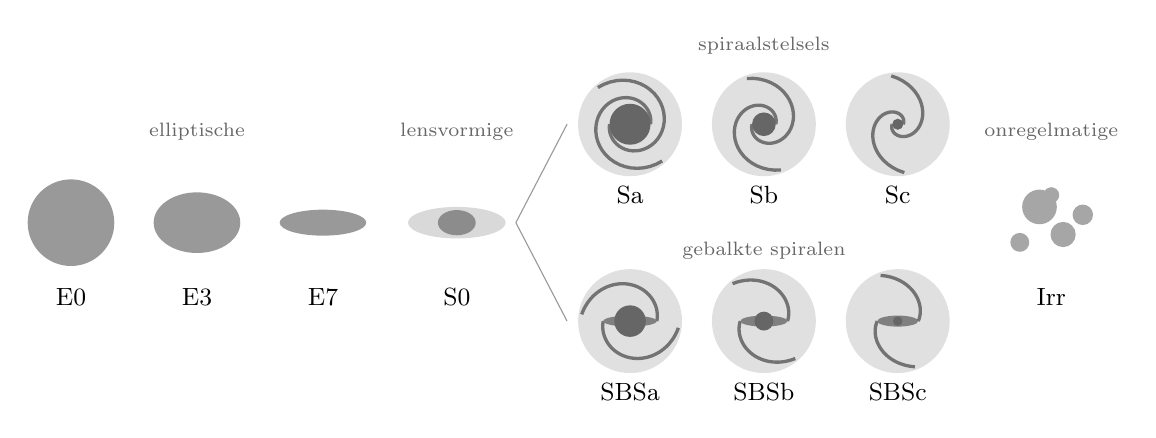
\begin{tikzpicture}[font=\small]
\def\spiralgal#1#2#3#4#5{% x, y, bulge radius, winding rate, bar half-length
  \begin{scope}[shift={(#1,#2)}]
    \fill[black!12] (0,0) circle (0.66);
    \pgfmathsetmacro{\rs}{max(#3,#5)}
    \pgfmathsetmacro{\th}{ln(0.62/\rs)/#4}
    \foreach \a in {0,180}
      \draw[line width=1.2pt, black!55, rotate=\a]
        plot[domain=0:\th, samples=40] ({\rs*exp(#4*\x)*cos(\x r)}, {\rs*exp(#4*\x)*sin(\x r)});
    \ifdim #5pt>0pt \fill[black!50] (0,0) ellipse (#5 and 0.07); \fi
    \fill[black!60] (0,0) circle (#3);
  \end{scope}}
\fill[black!40] (0,0) circle (0.55);
\fill[black!40] (1.6,0) ellipse (0.55 and 0.385);
\fill[black!40] (3.2,0) ellipse (0.55 and 0.165);
\fill[black!15] (4.9,0) ellipse (0.62 and 0.20);
\fill[black!45] (4.9,0) ellipse (0.24 and 0.16);
\draw[black!40] (5.65,0) -- (6.3,1.25);
\draw[black!40] (5.65,0) -- (6.3,-1.25);
\spiralgal{7.1}{1.25}{0.26}{0.16}{0}
\spiralgal{8.8}{1.25}{0.15}{0.28}{0}
\spiralgal{10.5}{1.25}{0.07}{0.45}{0}
\spiralgal{7.1}{-1.25}{0.20}{0.20}{0.34}
\spiralgal{8.8}{-1.25}{0.12}{0.32}{0.30}
\spiralgal{10.5}{-1.25}{0.06}{0.45}{0.26}
\foreach \p/\r in {(12.3,0.2)/0.22,(12.6,-0.15)/0.16,(12.05,-0.25)/0.12,(12.45,0.35)/0.1,(12.85,0.1)/0.13}
  \fill[black!35] \p circle (\r);
\foreach \x/\t in {0/E0,1.6/E3,3.2/E7,4.9/S0}
  \node at (\x,-0.95) {\t};
\foreach \x/\t in {7.1/Sa,8.8/Sb,10.5/Sc}
  { \node at (\x,0.35) {\t}; \node at (\x,-2.15) {SB\t}; }
\node at (12.45,-0.95) {Irr};
\node[font=\scriptsize, black!60] at (1.6,1.15) {elliptische};
\node[font=\scriptsize, black!60] at (4.9,1.15) {lensvormige};
\node[font=\scriptsize, black!60] at (8.8,2.25) {spiraalstelsels};
\node[font=\scriptsize, black!60] at (8.8,-0.35) {gebalkte spiralen};
\node[font=\scriptsize, black!60] at (12.45,1.15) {onregelmatige};
\end{tikzpicture}
\par\smallskip{\small De \omterm{def:b3:milky-way-galaxies:types}{Hubble-reeks}, schematisch als stemvork getekend,
Elliptische sterrenstelsels worden naar hun schijnbare afplatting benoemd;
de vork vertakt zich bij de lensvormige stelsels in gewone en gebalkte spiralen,
geordend van grote bulges en strak opgerolde armen (a) tot kleine bulges en
open armen (c); onregelmatige stelsels sluiten de reeks af.}\label{fig:b3:milky-way-galaxies:fork}
\end{omfigure}
% ledger: buta11:hubble

De klassen beschrijven vormen die aan de hemel worden waargenomen, en één label verbergt een
bereik: een \omterm{def:b3:milky-way-galaxies:types}{elliptisch sterrenstelsel} dat langs zijn kortste as wordt gezien, lijkt rond, wat zijn
werkelijke afplatting ook is, en de grenzen tussen naburige klassen zijn een
kwestie van oordeel. In een catalogus van de sterrenstelsels in onze omgeving staat de
Melkweg vermeld als S(B)bc, een spiraal tussen Sb en Sc met een balk; haar grote
buur Andromeda (M31) is een Sb, het Triangulum-stelsel (M33) een Sc, en
de Grote en Kleine Magellaanse Wolken zijn onregelmatige stelsels.
% ledger: buta11:hubble, mcconn12:local-group

\begin{omfigure}
\centering
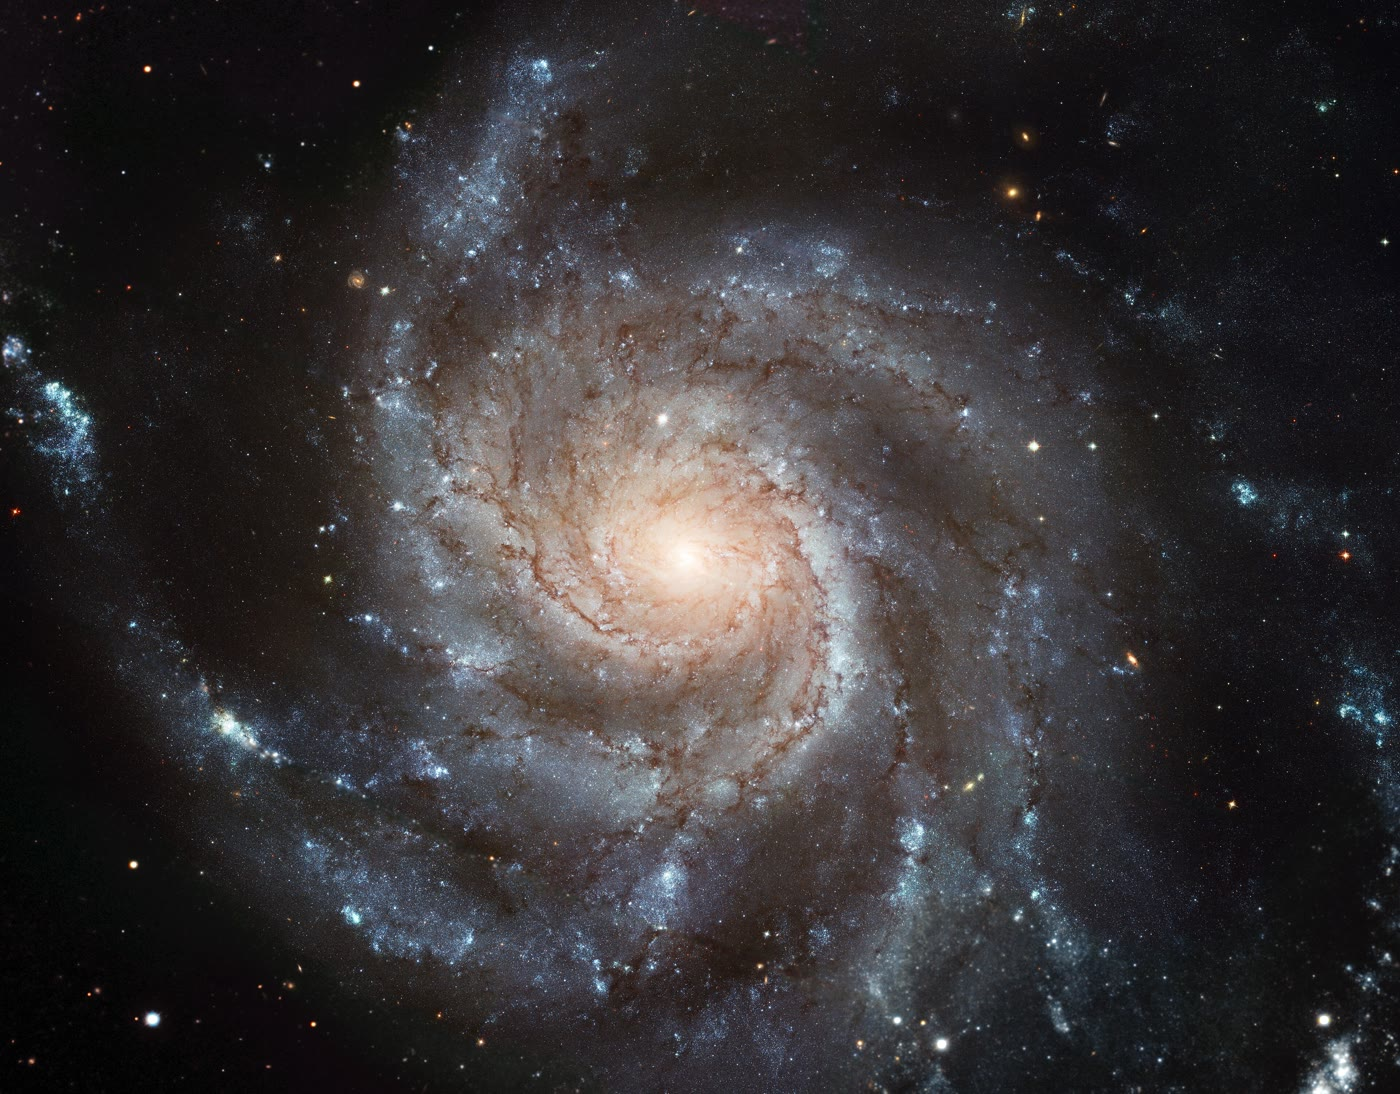
\includegraphics[width=0.66\linewidth]{images/book5/b3-m101.jpg}
\par\smallskip{\small Het \omterm{def:b3:milky-way-galaxies:types}{spiraalstelsel} M101, van bovenaf gezien door de Hubble
Space Telescope, een mozaïek van 51 opnamen, aan de randen bijgesneden: een kleine,
heldere, geelachtige bulge; open armen, blauwer en doorspekt met clusters van
jonge sterren; bruine stofbanen langs de armen. Beeld ESA en NASA
(Hubble, heic0602), CC BY~4.0.}\label{fig:b3:milky-way-galaxies:m101}
\end{omfigure}
% ledger: photo:b3-m101

Waarom zijn spiraalarmen niet opgerold? In een schijf waarvan de \omterm{def:b3:milky-way-galaxies:rotation-curve}{rotatiekromme} vlak is,
een ster op half de afstand van het centrum draait in de halve tijd rond.
Een spiraal van sterren zou bij elke omwenteling strakker worden opgerold, en na enkele
omwentelingen van de schijf zou het een strakke spoel zijn (zie \cref{exo:b3:milky-way-galaxies:11}).

\begin{definition}[Dichtheidsgolftheorie]\label{def:b3:milky-way-galaxies:density-wave}
De \emph{dichtheidsgolftheorie}\index{dichtheidsgolftheorie} verklaart spiraalarmen
als een golf van hogere dichtheid in een schijf, een spiraalpatroon dat
stijf draait met zijn eigen hoeksnelheid, de patroonsnelheid, terwijl de sterren en
het gas erdoorheen bewegen, vertragend bij het binnengaan van de drukke arm en
versnellend bij het verlaten ervan, zoals auto's door een file rijden.
\end{definition}

De theorie, in 1964 voorgesteld, verlost de armen van het oprolprobleem.
Gas dat een arm binnenkomt wordt samengeperst, en daar ontstaan sterren: de armen worden
afgetekend door jonge sterren en gloeiend gas, terwijl de oude sterren veel
gelijkmatiger verdeeld zijn. Of de armen langlevende golven zijn, is nog altijd omstreden;
computersimulaties van schijven laten vaker armen groeien die tijdelijk zijn,
die oplossen en opnieuw vormen, en een passerend sterrenstelsel of een balk kan een
tweearmige spiraal aandrijven.
% ledger: dobbs14:density-wave

\begin{definition}[Superzwaar zwart gat]\label{def:b3:milky-way-galaxies:smbh}
Een \emph{supermassief zwart gat}\index{supermassief zwart gat} is een zwart
gat van een miljoen zonsmassa's of meer in het centrum van een sterrenstelsel.
\end{definition}

In het centrum van de Melkweg zit de compacte radiobron Sagittarius~A*
(Sgr~A*) tussen sterren op strakke, snelle banen. Om die banen te verklaren
is een centrale massa nodig van ongeveer vier miljoen zonsmassa's,
$\num[separate-uncertainty=true]{4.2 \pm 0.2 e6}$ zonsmassa's volgens een overzicht van de metingen. Sgr~A* beweegt nauwelijks
ten opzichte van verre sterrenstelsels: na aftrek van de baan van de Zon
bedraagt de resterende beweging hooguit enkele kilometers per seconde, dus
bevat hij minstens een kwart van die massa. Zijn grootte is vergelijkbaar
met zijn Schwarzschildstraal, en zijn dichtheid, boven \num{4e23} zonsmassa's
per kubieke parsec, ligt zeer dicht bij wat voor een zwart gat wordt verwacht:
het bewijs dat Sgr~A* er een is, is overweldigend.
% ledger: reid20:sgra, bhg16:structure, gravity19:r0

\begin{definition}[Lokale Groep; cluster van sterrenstelsels]\label{def:b3:milky-way-galaxies:groups}
De \emph{Lokale Groep}\index{Lokale Groep} is de door zwaartekracht gebonden
groep van sterrenstelsels, gedomineerd door de Melkweg en Andromeda, elk met
hun satellietstelsels. Een \emph{cluster van sterrenstelsels}\index{cluster van sterrenstelsels} is
een van de grootste door zwaartekracht gebonden systemen: vele sterrenstelsels
bijeengehouden, met een heet gas dat röntgenstraling uitzendt, in een gemeenschappelijke
put van grotendeels donkere materie.
\end{definition}

Meer dan honderd sterrenstelsels bevinden zich binnen \qty{3}{Mpc} van de Zon, de meeste
daarvan dwergstelsels. De Grote Magellaanse Wolk staat op ongeveer \qty{50}{kpc}, Andromeda op
\qty{783}{kpc} en nadert ons met \qty{300}{km.s^{-1}}, en de gebonden
leden van de groep liggen binnen ongeveer \qty{1.06}{Mpc} van hun zwaartepunt,
tussen de Melkweg en Andromeda, waar zij zich afkeren van de
uitdijing van het heelal. De massa, afgeleid uit de beweging van de twee grote
sterrenstelsels naar elkaar toe, is van de orde van \num{5e12} zonsmassa's. In een
massieve \omterm{def:b3:milky-way-galaxies:groups}{cluster van sterrenstelsels} bedraagt het hete gas, bij ongeveer \qty{e8}{K},
ongeveer tien keer de massa van de sterren; sterrenstelsels en gas samen zijn te licht voor
de diepte van de zwaartekrachtput, en het grootste deel van de massa van de cluster,
van de orde van \num{e15} zonsmassa's, is donker.
% ledger: mcconn12:local-group, kravtsov12:clusters

\section{De afstandsladder}\label{sec:b3:milky-way-galaxies:ladder}

Een parallax geeft een afstand uitsluitend op grond van meetkunde, maar parallaxen worden kleiner naarmate de afstand toeneemt. De beste catalogus daarvan meet een parallax met een
onzekerheid van 0.02 tot \qty{0.03}{mas} voor sterren helderder dan
magnitude~15, zodat een afstand met een nauwkeurigheid van \qty{10}{\percent} tot ongeveer
\qty{4}{kpc} mogelijk is; de Grote Magellaanse Wolk, op \qty{50}{kpc}, heeft een
parallax van \qty{0.02}{mas}. Verder rusten afstanden op
objecten waarvan de
lichtkracht bekend is.
% ledger: gaia:dr3, freedman19:trgb

\begin{definition}[Standaardkaars; afstandsladder]\label{def:b3:milky-way-galaxies:ladder}
Een \emph{standaardkaars}\index{standaardkaars} is een klasse van objecten
waarvan de absolute magnitude bekend is, of kan worden afgeleid uit een eigenschap
die onafhankelijk van de afstand is gemeten, zodat hun schijnbare magnitude
hun afstandsmodulus geeft. De \emph{afstandsladder}\index{afstandsladder} is
de keten van methoden, elk gekalibreerd op objecten die dichtbij genoeg zijn om
ook met de voorgaande methode te worden gemeten, die afstanden vanuit
parallaxen uitbreidt tot het uitdijende heelal.
\end{definition}

\begin{definition}[Cepheïde; wet van Leavitt]\label{def:b3:milky-way-galaxies:cepheid}
Een \emph{cepheïde}\index{cepheïde} is een jonge, lichtkrachtige, pulserende
ster waarvan de helderheid varieert met een strikt regelmatige periode,
van ongeveer een dag tot enkele weken. De \emph{wet van Leavitt}\index{wet van Leavitt},
of periode--lichtkrachtrelatie, is het lineaire verband tussen de gemiddelde
absolute magnitude van een cepheïde en de logaritme van haar periode, waarbij
langere perioden horen bij helderdere sterren.
\end{definition}

Het verband werd in 1908 ontdekt in de Kleine Magellaanse Wolk, waarvan de sterren
allemaal op nagenoeg dezelfde afstand staan. Stof in het sterrenstelsel waarin een \omterm{def:b3:milky-way-galaxies:cepheid}{cepheïde} staat,
dimt en rood-kleurt haar; maar de dimming is groter in het zichtbare dan in het
nabije infrarood, in een vaste verhouding voor een bepaald soort stof, en de combinatie
$W_I = I - 1.55\,(V - I)$ van de magnitudes in de I- en V-banden, de Wesenheit-index, is zo gekozen dat de dimming
wegvalt. De figuur hieronder toont dit voor 2315 \omterm{def:b3:milky-way-galaxies:cepheid}{cepheïden}
van de Grote Magellaanse Wolk:
de \omterm{def:b3:milky-way-galaxies:cepheid}{wet van Leavitt} is een strakke lijn, met een spreiding van
\qty{0.078}{mag}, dat is \qty{3.6}{\percent} in afstand voor één
ster.
% ledger: sos15:leavitt, data:b5-ogle-lmc-cep

\begin{omfigure}
\centering
\begin{tikzpicture}
\begin{axis}[width=0.80\linewidth, height=0.52\linewidth,
  xmin=-0.05, xmax=1.6, ymin=10, ymax=16.6, y dir=reverse,
  xlabel={$\log_{10}(P/\mathrm{d})$}, ylabel={Wesenheit-index $W_I$ (mag)},
  tick label style={font=\scriptsize}, label style={font=\small},
  legend style={font=\scriptsize, at={(0.5,-0.17)}, anchor=north, legend columns=3, draw=none, cells={anchor=west}, /tikz/every even column/.append style={column sep=1em}},
  legend image post style={scale=2.2}]
\addplot[only marks, mark=*, mark size=0.45pt, omDef, opacity=0.6] table[x=logp, y=w] {figdata/out/bachelor-3-distance_ladder-pl.dat};
\addlegendentry{cepheïden}
\addplot[only marks, mark=x, mark size=1.6pt, red!70!black] table[x=logp, y=w] {figdata/out/bachelor-3-distance_ladder-clipped.dat};
\addlegendentry{buitengesloten ($>3\sigma$)}
\addplot[thick, black] table[x=logp, y=w_fit] {figdata/out/bachelor-3-distance_ladder-fit.dat};
\addlegendentry{fit}
\node[font=\scriptsize, anchor=south west, fill=white, inner sep=1pt] at (axis cs:0.55,11.0) {$W_I = -3.315\log_{10}P + 15.889$};
\end{axis}
\end{tikzpicture}
\par\smallskip{\small De \omterm{def:b3:milky-way-galaxies:cepheid}{wet van Leavitt} in de Grote Magellaanse Wolk:
de Wesenheit-index van 2315 \omterm{def:b3:milky-way-galaxies:cepheid}{cepheïden} die pulseren in hun fundamentele modus
tegen de logaritme van hun periode (OGLE-survey, Soszyński en
anderen, 2015, via de CDS). Helderdere sterren liggen hoger. Een rechte lijn
door de kleinste kwadraten, na het terzijde zetten van 92 sterren die meer dan
drie standaarddeviaties ervan afliggen, reproduceert de gepubliceerde relatie
($-3.314$, $15.888$). Met de afstandsmodulus van de Wolk, 18.477, geeft de lijn
de absolute Wesenheit-magnitude van elke \omterm{def:b3:milky-way-galaxies:cepheid}{cepheïde} uit haar periode.}\label{fig:b3:milky-way-galaxies:leavitt}
\end{omfigure}
% ledger: data:b5-ogle-lmc-cep, sos15:leavitt, freedman19:trgb

\begin{definition}[Top van de rode-reuzentak]\label{def:b3:milky-way-galaxies:trgb}
De \emph{top van de rode-reuzentak}\index{top van de rode-reuzentak}
(TRGB) is de scherpe bovengrens van de helderheden van de rode reuzen van
een oude \omterm{def:b3:milky-way-galaxies:populations}{sterpopulatie}, bepaald door de ontsteking van helium in hun kernen,
de heliumflits; in de I-band ligt hij op vrijwel dezelfde absolute
magnitude in elke oude populatie, $M_I \approx -4.05$ bij een kleur
$V - I = 1.6$, en hangt maar zwak af van de chemische samenstelling.
\end{definition}

De top wordt gemeten in de ijle halo's van sterrenstelsels, waar weinig stof
is en weinig verdringing; hij gebruikt oude halosterren waar \omterm{def:b3:milky-way-galaxies:cepheid}{cepheïden}
jonge schijfsterren gebruiken, en de twee methoden delen geen natuurkunde. \omterm{def:b3:milky-way-galaxies:cepheid}{Cepheïden} en
de TRGB reiken tot enkele tientallen megaparsec, tot in sterrenstelsels waar een
zeldzame en veel helderdere \omterm{def:b3:milky-way-galaxies:ladder}{standaardkaars} is ontploft: een supernova van type~Ia,
de thermonucleaire explosie van een witte dwerg, bekend uit de natuurkundeboeken,
waarvan de piekabsolute magnitude, na correctie voor de
vorm van zijn lichtkromme en zijn kleur, is
$M_B = \qty[separate-uncertainty=true]{-19.253 \pm 0.027}{mag}$. Zulke
supernova's zijn over honderden megaparsec waar te nemen.
% ledger: freedman19:trgb, riess22:h0

\begin{definition}[Tully--Fisher-relatie]\label{def:b3:milky-way-galaxies:tully-fisher}
De \emph{Tully--Fisher-relatie}\index{Tully--Fisher-relatie} is de
correlatie tussen de helderheid, of beter de massa van sterren en gas,
van een \omterm{def:b3:milky-way-galaxies:types}{spiraalstelsel} en de snelheid van zijn vlakke \omterm{def:b3:milky-way-galaxies:rotation-curve}{rotatiekromme}; in zijn
baryonische vorm, $M_\mathrm{b} = A\,V^4$, geldt ze van ongeveer 30 tot
\qty{300}{km.s^{-1}}.
\end{definition}

Het 21-cm-spectrum van een sterrenstelsel geeft zijn maximale rotatiesnelheid, de
relatie zijn helderheid, onafhankelijk van zijn afstand, en zijn flux
geeft dan de afstand: een sport voor \omterm{def:b3:milky-way-galaxies:types}{spiraalstelsels} die te ver weg zijn voor afzonderlijke
sterren. De Melkweg valt door zijn helderheid en rotatie op de relatie.
% ledger: mcgaugh00:btf, nrao:hi-line, bhg16:structure

\begin{omfigure}
\centering
\pgfplotstableread{figdata/out/bachelor-3-distance_ladder-ladder.dat}\laddertab
\pgfplotstableread{figdata/out/bachelor-3-distance_ladder-anchors.dat}\anchortab
\pgfplotstablegetelem{0}{d_hi}\of{\laddertab}\let\plxhi\pgfplotsretval
\pgfplotstablegetelem{1}{d_lo}\of{\laddertab}\let\cephlo\pgfplotsretval
\pgfplotstablegetelem{1}{d_hi}\of{\laddertab}\let\cephhi\pgfplotsretval
\pgfplotstablegetelem{3}{d_lo}\of{\laddertab}\let\snlo\pgfplotsretval
\pgfplotstablegetelem{3}{d_hi}\of{\laddertab}\let\snhi\pgfplotsretval
\pgfplotstablegetelem{1}{d}\of{\anchortab}\let\mthirtyone\pgfplotsretval
\pgfplotstablegetelem{2}{d}\of{\anchortab}\let\nfourtwo\pgfplotsretval
\begin{tikzpicture}
\begin{axis}[width=0.92\linewidth, height=0.42\linewidth,
  xmode=log, xmin=1e-3, xmax=2e6, ymin=0.4, ymax=4.9,
  ytick={1,2,3,4}, yticklabels={parallaxen, cepheïden, TRGB, SNe~Ia},
  xtick={1e-3,1e-2,1e-1,1,10,100,1e3,1e4,1e5,1e6},
  xticklabels={1\,pc,,,1\,kpc,,,1\,Mpc,,,1\,Gpc},
  xlabel={afstand}, tick label style={font=\scriptsize}, label style={font=\small},
  y tick label style={font=\small}, axis y line*=left, axis x line*=bottom]
\draw[line width=7pt, omDef!70] (axis cs:1e-3,1) -- (axis cs:\plxhi,1);
\draw[line width=7pt, omMeth!70] (axis cs:\cephlo,2) -- (axis cs:\cephhi,2);
\draw[line width=7pt, omProp!70] (axis cs:\cephlo,3) -- (axis cs:\cephhi,3);
\draw[line width=7pt, red!60] (axis cs:\snlo,4) -- (axis cs:\snhi,4);
\draw[densely dotted, thick] (axis cs:\cephlo,0.4) -- (axis cs:\cephlo,4.55) node[anchor=south, font=\scriptsize] {LMC};
\draw[densely dotted, thick] (axis cs:\mthirtyone,0.4) -- (axis cs:\mthirtyone,4.55) node[anchor=south, font=\scriptsize] {M31};
\draw[densely dotted, thick] (axis cs:\nfourtwo,0.4) -- (axis cs:\nfourtwo,4.55) node[anchor=south, font=\scriptsize] {NGC~4258};
\draw[->, thick, black!60] (axis cs:\plxhi,1.25) to[out=30, in=200] (axis cs:\cephlo,1.75);
\draw[->, thick, black!60] (axis cs:\cephhi,2.25) to[out=40, in=220] (axis cs:\snlo,3.75);
\end{axis}
\end{tikzpicture}
\par\smallskip{\small De sporten van de \omterm{def:b3:milky-way-galaxies:ladder}{afstandsladder}, met de
afstanden waarover elke sport hier wordt gebruikt: parallaxen van de beste catalogus,
tot \qty{10}{\percent} uit tot \qty{4}{kpc}; \omterm{def:b3:milky-way-galaxies:cepheid}{cepheïden} en de TRGB vanaf de
Grote Magellaanse Wolk tot de gastheren van de dichtstbijzijnde supernova's van type~Ia,
\qty{45}{Mpc}; de supernova's van de gladde expansie, bij roodverschuivingen van 0.023
tot 0.15 (\qtyrange{96}{616}{Mpc} voor $H_0 = 73$). Stippellijnen: twee ankers van
de cepheïdenschaal met geometrische afstanden (bedekkingsdubbelsterren in de
Grote Magellaanse Wolk, watermasers die het zwarte gat van NGC~4258 omcirkelen), en M31, het
dichtstbijzijnde grote \omterm{def:b3:milky-way-galaxies:types}{spiraalstelsel}. Pijlen: elke sport wordt geijkt op objecten die de
sport eronder ook meet, de \omterm{def:b3:milky-way-galaxies:cepheid}{cepheïden} van de Melkweg via hun parallaxen,
de supernova's van nabije sterrenstelsels via de \omterm{def:b3:milky-way-galaxies:cepheid}{cepheïden} en de TRGB van hun
gastheren.}\label{fig:b3:milky-way-galaxies:ladder-rungs}
\end{omfigure}
% ledger: gaia:dr3, riess22:h0, freedman19:trgb, mcconn12:local-group

Bovenaan de ladder meten de supernova's de expansie van het
heelal. De wet van Hubble, bekend uit de natuurkundeboeken, maakt de
recessiesnelheid $cz$ van een ver sterrenstelsel evenredig met zijn afstand $d$,
$cz = H_0 d$ voor kleine roodverschuivingen $z$; de Hubble-constante $H_0$ is de
helling, en de supernova's geven die, met hun afstanden uit de ladder.

\begin{definition}[Hubble-spanning]\label{def:b3:milky-way-galaxies:tension}
De \emph{Hubble-spanning}\index{Hubble-spanning} is het verschil tussen de
waarde van de Hubble-constante die lokaal is gemeten met de
\omterm{def:b3:milky-way-galaxies:ladder}{afstandsladder} en de waarde die is afgeleid uit de kosmische
achtergrondstraling met het standaardmodel van de kosmologie.
\end{definition}

\begin{dated}{2022}
De \omterm{def:b3:milky-way-galaxies:cepheid}{cepheïden} van de gastheren van 42 supernova's van type~Ia, verankerd op
parallaxen, de masers van NGC~4258 en de bedekkingsdubbelsterren van de
Grote Magellaanse Wolk geven
$H_0 = \qty[separate-uncertainty=true]{73.04 \pm 1.04}{km.s^{-1}.Mpc^{-1}}$.
De \omterm{def:b3:milky-way-galaxies:trgb}{top van de rode-reuzentak}, die ongeveer honderd supernova's ijkt,
gaf in 2019 $H_0 = 69.8 \pm 0.8 \pm \qty{1.7}{km.s^{-1}.Mpc^{-1}}$
(statistisch en systematisch). De kaart van de kosmische
achtergrondstraling van de Planck-satelliet, gelezen met het standaardmodel van de kosmologie, impliceert
$H_0 = \qty[separate-uncertainty=true]{67.4 \pm 0.5}{km.s^{-1}.Mpc^{-1}}$.
De cepheïdewaarde en de waarde uit de achtergrond verschillen met vijf standaardafwijkingen;
de TRGB-waarde ligt daartussen. De oorsprong van het
verschil is niet bekend: een fout die nog niet is gevonden in een van de ladders,
of natuurkunde die in het model ontbreekt.
\end{dated}
% ledger: riess22:h0, freedman19:trgb, planck18:h0

\begin{inthelab}[Een astrometrische satelliet en zijn catalogus]
De satelliet Gaia scant de hemel volgens een vooraf vastgelegd patroon, zodat elke
ster tijdens de missie steeds opnieuw wordt gemeten. Op de grond zetten de
coördinatie-eenheden van een consortium voor gegevensverwerking deze
metingen om in een positie, een parallax en een eigenbeweging voor elk van
meer dan een miljard bronnen: van de kleine bewegingen van een ster aan de hemel
is de parallax het deel dat zich elk jaar herhaalt en de eigenbeweging
het deel dat zich opstapelt. Elke catalogus wordt uitgebracht met artikelen die
de verwerking en de validatie ervan beschrijven, en elke afstand in de
figuren van deze paragraaf die op een parallax berust, berust op zo'n
catalogus.
\end{inthelab}

\begin{dated}{2022}
De derde Gaia-catalogus, uitgebracht op 13 juni 2022 op basis van 34 maanden
waarnemingen, geeft posities, parallaxen en eigenbewegingen voor ongeveer
1.46~miljard bronnen, van magnitude~3 tot~21, en gemiddelde radiale snelheden
voor 33~miljoen sterren. De onzekerheden in de parallax bedragen van 0.02 tot
\qty{0.03}{mas} voor sterren helderder dan magnitude~15, \qty{0.07}{mas} bij
magnitude~17, en \qty{0.5}{mas} bij magnitude~20.
\end{dated}
% ledger: gaia:dr3

\section{Oefeningen}

\begin{exercise}[$\star$]\label{exo:b3:milky-way-galaxies:1}
De galactische jaar van de Zon. (a)~Met $R_0 = \qty{8.178}{kpc}$ en
$V_0 = \qty{229}{km.s^{-1}}$, bereken de omlooptijd van de baan van de Zon om
het galactisch centrum, in miljoen jaar. (b)~Hoeveel keer is de Zon
rondgegaan sinds het Zonnestelsel is ontstaan, \qty{4.54}{Gyr} geleden?
\end{exercise}

\begin{exercise}[$\star$]\label{exo:b3:milky-way-galaxies:2}
De terugstotbeweging van Sgr~A*. (a)~Een eigenbeweging van \qty{1}{mas} per jaar
bij \qty{1}{kpc} komt overeen met een transversale snelheid van \qty{1}{au} per jaar: druk die uit in
kilometer per seconde. (b)~Sgr~A*, aangenomen in rust in het galactisch centrum
op \qty{8.178}{kpc}, drijft langs het galactische vlak met \qty{6.411}{mas}
per jaar. Bereken de snelheid van de Zon om het centrum en vergelijk die met de
waarde uit het overzicht, \qty[separate-uncertainty=true]{248 \pm 3}{km.s^{-1}}. (c)~Trek de
peculiere beweging van de Zon in de draairichting af, \qty{11}{km.s^{-1}}, en
vergelijk met $V_0$ uit de \omterm{def:b3:milky-way-galaxies:rotation-curve}{rotatiekromme}.
\end{exercise}

\begin{exercise}[$\star$]\label{exo:b3:milky-way-galaxies:3}
Elliptische sterrenstelsels indelen. (a)~De isofoten van een \omterm{def:b3:milky-way-galaxies:types}{elliptisch sterrenstelsel} hebben een
assenverhouding van 0.6: geef de klasse. (b)~Welke assenverhouding heeft een E7?
(c)~Waarom kan een E0-sterrenstelsel een afgeplat systeem zijn?
\end{exercise}

\begin{exercise}[$\star$]\label{exo:b3:milky-way-galaxies:4}
Ankers. Bereken de afstanden van de Grote Magelhaense Wolk
($\mu = 18.477$), Andromeda ($\mu = 24.47$) en NGC~4258
($\mu = 29.398$). Welke parallax zou een ster van de Wolk hebben, en waarom
kan de afstand van de Wolk niet met parallaxen worden gemeten?
\end{exercise}

\begin{exercise}[$\star\star$]\label{exo:b3:milky-way-galaxies:5}
Uit de \omterm{def:b3:milky-way-galaxies:rotation-curve}{Oort-constanten} $A = \qty{15.3}{km.s^{-1}.kpc^{-1}}$ en
$B = \qty{-11.9}{km.s^{-1}.kpc^{-1}}$: (a)~bereken de hoeksnelheid van
de LSR en, met $R_0 = \qty{8.178}{kpc}$, de cirkelsnelheid $V_0$;
(b)~bereken de helling van de \omterm{def:b3:milky-way-galaxies:rotation-curve}{rotatiekromme} bij de Zon. (c)~Vergelijk
met de \omterm{def:b3:milky-way-galaxies:rotation-curve}{rotatiekromme} van de rode reuzen ($V_0 = \qty{229.0}{km.s^{-1}}$,
helling \qty{-1.7}{km.s^{-1}} per kiloparsec) en verklaar waarom de twee
verschillen, gegeven dat dezelfde meting een niet-nulwaarde voor $C$ en $K$ vond.
\end{exercise}

\begin{exercise}[$\star\star$]\label{exo:b3:milky-way-galaxies:6}
Een vlakke \omterm{def:b3:milky-way-galaxies:rotation-curve}{rotatiekromme} en de lokale dichtheid. (a)~Voor een bolvormig sterrenstelsel
met een vlakke \omterm{def:b3:milky-way-galaxies:rotation-curve}{rotatiekromme} bij \qty{229}{km.s^{-1}}, bereken de dichtheid op
\qty{8.178}{kpc}, in zonsmassa's per kubieke parsec
($G = \qty{4.301e-6}{kpc.(km.s^{-1})^2}$ per zonsmassa). (b)~Toon aan dat
één zonsmassa per kubieke parsec \qty{37.96}{GeV.cm^{-3}} is, en druk
de lokale dichtheid van donkere materie, \qty{0.30}{GeV.cm^{-3}}, uit in zonsmassa's
per kubieke parsec. (c)~Waarom is de dichtheid van (a) groter?
\end{exercise}

\begin{exercise}[$\star\star$]\label{exo:b3:milky-way-galaxies:7}
Een cepheïde-afstand. In een verzonnen \omterm{def:b3:milky-way-galaxies:types}{spiraalstelsel} heeft een \omterm{def:b3:milky-way-galaxies:cepheid}{cepheïde} met een periode van
\qty{30}{d} een gemiddelde Wesenheit-index $W_I = \qty{25.00}{mag}$.
(a)~Gebruik de \omterm{def:b3:milky-way-galaxies:cepheid}{wet van Leavitt} van de Grote Magelhaense Wolk,
$W_I = -3.314\log_{10}P + 15.888$, en de afstandsmodulus van de Wolk
18.477, om de absolute Wesenheit-magnitude van de \omterm{def:b3:milky-way-galaxies:cepheid}{cepheïde} te berekenen. (b)~Bereken
de afstand van het sterrenstelsel. (c)~De spreiding van de wet is \qty{0.077}{mag}: wat is
de relatieve afstandsfout uit één \omterm{def:b3:milky-way-galaxies:cepheid}{cepheïde} en uit vijftig?
\end{exercise}

\begin{exercise}[$\star\star$]\label{exo:b3:milky-way-galaxies:8}
Een TRGB-afstand. In de halo van een verzonnen sterrenstelsel wordt de \omterm{def:b3:milky-way-galaxies:trgb}{top van de
rode-reuzentak} gevonden op $I = \qty{26.00}{mag}$; het stof langs de
zichtlijn dimt de I-band met \qty{0.05}{mag}. Bereken, met $M_I = -4.05$, de
afstandsmodulus en de afstand. Wat betekent een onzekerheid van
\qty{0.04}{mag} in de top voor de afstand?
\end{exercise}

\begin{exercise}[$\star\star$]\label{exo:b3:milky-way-galaxies:9}
De Hubble-constante uit supernova's. Voor een supernova van de gladde
expansie, $\log_{10}(cz) - 0.2\,m_B = a_B$, het snijpunt van het
Hubble-diagram van de supernova's, en de afstandsmodulus is
$m_B - M_B = 5\log_{10}(d/\mathrm{Mpc}) + 25$. (a)~Toon aan dat
$\log_{10}H_0 = 0.2\,M_B + a_B + 5$ ($H_0$ in kilometer per seconde per
megaparsec). (b)~Met $M_B = -19.253$ en $a_B = 0.714158$, bereken $H_0$.
(c)~Welke $M_B$ zou $H_0 = \qty{67.4}{km.s^{-1}.Mpc^{-1}}$ geven? Met hoeveel
magnitudes, en met welk deel van de afstanden, verschillen de twee
ijkingen?
\end{exercise}

\begin{exercise}[$\star\star\star$]\label{exo:b3:milky-way-galaxies:10}
Waar de wet van Tully--Fisher vandaan komt. (a)~Een schijfstelsel met massa $M$
en straal $R$ draait met $V$: toon aan dat $M \approx RV^2/G$. (b)~Als alle
\omterm{def:b3:milky-way-galaxies:types}{spiraalstelsels} dezelfde gemiddelde oppervlaktedichtheid $\Sigma = M/(\pi R^2)$ hadden,
toon dan aan dat $M \propto V^4$. (c)~Twee verzonnen sterrenstelsels op dezelfde baryonische
relatie draaien met 100 en \qty{229}{km.s^{-1}}: wat is de verhouding van
hun massa's? (d)~Twee sterrenstelsels draaien met dezelfde snelheid en hebben dezelfde
lichtkracht; het ene geeft vier keer de flux van het andere. Vergelijk hun
afstanden.
\end{exercise}

\begin{exercise}[$\star\star\star$]\label{exo:b3:milky-way-galaxies:11}
Het wikkelprobleem. Een schijf draait met een vlakke \omterm{def:b3:milky-way-galaxies:rotation-curve}{rotatiekromme} bij
\qty{229}{km.s^{-1}}. (a)~Reken deze snelheid om naar kiloparsec per miljard
jaar. (b)~Een rechte arm van sterren loopt op tijdstip nul van 4 tot
\qty{12}{kpc}. Bereken de omloopperiodes aan beide uiteinden. (c)~Na
\qty{1}{Gyr}, over welke hoek is het binnenste uiteinde voorop gegaan ten opzichte van het buitenste
uiteinde? Hoeveel windingen van een spiraal is dat, en hoe zou de arm
eruitzien? (d)~Hoe ontloopt een dichtheidsgolf dit?
\end{exercise}

\begin{exercise}[$\star\star\star$]\label{exo:b3:milky-way-galaxies:12}
Het zwarte gat in het centrum. Neem voor de centrale massa
\num{4.2e6} zonsmassa's en $R_0 = \qty{8178}{pc}$. (a)~De ster S2
draait er in \num{16}~jaar omheen: bereken de halve lange as van zijn baan
in astronomische eenheden (de derde wet van Kepler in zonne-eenheden, $a^3 = MP^2$ met
$a$ in au, $P$ in jaar en $M$ in zonsmassa's) en zijn hoekgrootte gezien
vanaf de Aarde. (b)~Bereken de Schwarzschild-straal van het zwarte gat in meter
en in astronomische eenheden, en de hoek die zijn diameter vanaf de Aarde
onderspant, in microboogseconden. (c)~Bereken de gemiddelde dichtheid van de massa
binnen zijn Schwarzschild-straal, in zonsmassa's per kubieke parsec, en
vergelijk die met de ondergrens die de beweging van Sgr~A* stelt,
\num{4e23} zonsmassa's per kubieke parsec.
\end{exercise}

\section{Probleem: De Melkweg wegen}

\begin{problem}[{Weekendprobleem --- van de bewegingen van sterren en gas tot
de donkere materie binnen \qty{20}{kpc}}]
\label{pb:b3:milky-way-galaxies:1}
Neem $R_0 = \qty{8.18}{kpc}$, $G = \qty{4.301e-6}{kpc.(km.s^{-1})^2}$ per
zonsmassa, en \qty{4.74}{km.s^{-1}} voor een eigenbeweging van
\qty{1}{mas} per jaar bij \qty{1}{kpc}. Alle snelheden zijn ten opzichte van de
LSR. Gebruik de stellingen van Oort en die van het raakpunt uit het hoofdstuk, en de
bolsymmetrische benadering $M = RV^2/G$ voor dynamische massa's.

\medskip\noindent\textbf{Deel I --- De lokale rotatie.} Een verzonnen
onderzoek naar roodeklompsterren, allemaal op $d = \qty{1.00}{kpc}$ in het galactische
vlak, geeft een gemiddelde radiale snelheid van \qty{+15.4}{km.s^{-1}} bij
$\ell = \ang{45}$ en \qty{-15.2}{km.s^{-1}} bij $\ell = \ang{135}$, en
gemiddelde eigenbewegingen in lengte van \qty{-5.91}{mas} per jaar bij
$\ell = \ang{90}$ en \qty{+0.55}{mas} per jaar bij $\ell = \ang{0}$.
\begin{enumerate}
\item Wat voorspelt de formule van Oort voor de radiale snelheden bij
  $\ell = \ang{45}$, \ang{90}, \ang{135} en \ang{180}?
\item Bereken $A$ uit de twee radiale snelheden.
\item Bereken $B$ uit de eigenbeweging bij $\ell = \ang{90}$.
\item Bereken $B$ opnieuw uit de eigenbeweging bij $\ell = \ang{0}$, en
  vergelijk.
\item Bereken de hoeksnelheid van de LSR en de cirkelsnelheid
  $V_0$.
\item Bereken de helling van de \omterm{def:b3:milky-way-galaxies:rotation-curve}{rotatiekromme} ter plaatse van de Zon. Is de kromme
  stijgend, vlak of dalend?
\item Bereken de omloopperiode van de Zon en het aantal omwentelingen in
  \qty{4.54}{Gyr}.
\end{enumerate}

\medskip\noindent\textbf{Deel II --- De binnenste rotatiekromme.} Neem
$V_0 = \qty{229}{km.s^{-1}}$. De hoogste radiale snelheden in de
21-cm-profielen bij $\ell = \ang{40}$, \ang{50}, \ang{60} en \ang{70} zijn
82.9, 55.6, 32.4 en \qty{14.9}{km.s^{-1}}.
\begin{enumerate}[resume]
\item Waarom heeft de raakpuntmethode $\ang{0} < \ell < \ang{90}$ nodig
  (of het spiegelkwadrant), en waarom faalt zij voorbij de zonnecirkel?
\item Bereken de straal van het raakpunt voor elke lengtegraad.
\item Bereken $V(R)$ bij elk raakpunt.
\item Hoeveel, in kilohertz, is de lijn van het gas in het raakpunt
  bij $\ell = \ang{40}$ verschoven ten opzichte van zijn rustfrequentie,
  \qty{1420.405751}{MHz}, en in welke richting?
\item Vergelijk met de kromme van de rode reuzen, die \qty{226.8}{km.s^{-1}}
  geeft bij \qty{5.27}{kpc} en \qty{229.6}{km.s^{-1}} bij \qty{7.22}{kpc}. Is de
  binnenste kromme stijgend, vlak of dalend?
\item Stel dat de snelheid in het raakpunt bij $\ell = \ang{40}$ gelijk zou zijn aan die van
  een puntmassa in het centrum die de Zon met $V_0$ meevoert, hoe groot zou die zijn?
  Wat zegt de vergelijking over de verdeling van de massa?
\end{enumerate}

\medskip\noindent\textbf{Deel III --- De zichtbare massa.} Gebruik het massamodel
uit het hoofdstuk, in eenheden van zonsmassa's en kiloparsec: een
bolling van Plummer $M = \num{1.067e10}$, $b = 0.3$; een dunne Miyamoto--Nagai-schijf
$M = \num{3.944e10}$, $a = 5.3$, $b = 0.25$; een dikke van dezelfde
massa met $a = 2.6$, $b = 0.8$.
\begin{enumerate}[resume]
\item Bereken de totale zichtbare massa van het model en vergelijk die met de
  gangbare waarde voor de sterrenmassa van de Melkweg, \qty[separate-uncertainty=true]{5 \pm 1 e10}{}
  zonsmassa's.
\item Bereken de cirkelsnelheid van de bolling alleen bij \qty{20}{kpc}.
\item Bereken die van de dunne en van de \omterm{def:b3:milky-way-galaxies:structure}{dikke schijf} bij \qty{20}{kpc}.
\item Bereken de cirkelsnelheid van alle zichtbare massa bij
  \qty{20}{kpc}.
\item Bereken hetzelfde bij $R_0$, en vergelijk met $V_0$.
\item Als alle zichtbare massa in het centrum geconcentreerd zou zijn, hoe groot zou
  de snelheid dan zijn bij \qty{20}{kpc}? Waarom ligt de waarde van het model er dicht bij?
\end{enumerate}

\medskip\noindent\textbf{Deel IV --- De donkere materie.} De rode reuzen
geven een cirkelsnelheid van \qty{200}{km.s^{-1}} bij \qty{20}{kpc}.
\begin{enumerate}[resume]
\item Bereken de dynamische massa binnen \qty{20}{kpc}.
\item Bereken de dynamische massa van de zichtbare materie binnen
  \qty{20}{kpc}.
\item Bereken de massa van donkere materie binnen \qty{20}{kpc}, en toon aan dat
  haar aandeel $1 - (V_\mathrm{vis}/V)^2$ is.
\item De NFW-halo, gepast op de hele kromme, heeft
  $\rho_0 = \num{1.06e7}$ zonsmassa's per kubieke kiloparsec en
  $R_s = \qty{14.8}{kpc}$. Bereken de massa ervan binnen \qty{20}{kpc} en het
  donkere aandeel dat het daaruit volgt. Waarom wijkt dit af van het vorige antwoord?
\item Bereken de dichtheid van die halo bij $R_0$, in zonsmassa's per
  kubieke parsec en in \unit{GeV.cm^{-3}} (één zonsmassa per kubieke parsec
  is \qty{37.96}{GeV.cm^{-3}}).
\item Geef het aandeel donkere materie in de massa binnen \qty{20}{kpc}
  dat uit de gemeten snelheid volgt, in procent, op twee
  significante cijfers.
\end{enumerate}
\end{problem}
% ledger: gravity19:r0, eilers19:table1, pouliasis17:model1, eilers19:halo, bhg16:structure, nrao:hi-line, const:G, const:au, iau:parsec, usgs:age-earth
